\section{Stakeholders}
In het vooronderzoek wordt er een stakeholdersanalyse gemaakt om de stakeholders in beeld te krijgen.
De stakeholders zijn individuen of organisaties die invloed of belang hebben bij het project.
Somige exterene stakeholders zullen gereprenseerd worden door een gekwalificeerde interne medewerker van Snakeware.
Dit wordt gedaan omdat de afstudeer opdracht een proof of concept is, en de klanten van Snakware hier nog niet bij betrokken worden. 
Als na de afstudeerperiode het een success blijkt te zijn en Snakeware wilt het verder ontwikkelen dan wordt concact opgezocht met de externe stakeholders.
\subsection{Interne Stakeholders}
\todo[inline]{inleidend stukje text}
\todo[inline]{ik ben het ontwikkelteam volgens mij}
\begin{tabular}{ | p{4cm} | p{9cm} | }
	\hline
	\textbf{Stakeholder} & \textbf{Beschrijving}                                                                                                                      \\
	\hline
	Opdrachtgever       & De opdrachtgever overziet het project en fasiliteerd de communicatie tussen de ontwikkelaars en de klanten                                 \\
	\hline
	Afdeling R\&D        & de afdeling R\&D van Snakeware zijn de ontwikkelaars van het huidige CMS en kunnen veel inzicht bieden in de huidige situatie / problemen. \\
	\hline
	Developers           & Aan het einde van de afstudeerperiode moet het project overgedragen worden aan de developers van Snakeware.                                \\
	\hline
	Ontwikkelteam        & Het ontwikkelteam is verantwoordelijk voor het realiseren van het proof of concept                                                         \\
	\hline
\end{tabular}
\subsection{Externe Stakeholders}
\todo[inline]{inleidend stukje text}
\todo[inline]{Stakeholders beperken tot kleine,enterpriese en misschien Eindgebruikers (zijn deze nogsteeds exterern omdat ze worden gereperenseerd door interne mensen)?}
\begin{tabular}{ | p{4cm} | p{9cm} | }
	\hline
	\textbf{Stakeholders} & \textbf{Beschrijving}                                                                                                                                                           \\
    \hline
	Kleine klanten        & Dit zijn de klanten die nu nog niet groot genoeg zijn om een web applicatie aftesluiten bij Snakeware.                                                                          \\
	\hline
	Enterprise klanten    & Dit zijn klanten bij Snakeware die een grote hoeveelheid klanten heeft en meestal binnen Snakeware eigen teams heeft, Hierbij kan je denken aan Poieze, DRG en Rederij Doeksen. \\
	% \hline
	% Huidige klanten       & De huidige klanten die bij Snakeware een web applicatie hebben.                                                                                                                 \\
	\hline
	Eindgebruikers        & De personen die de content van de verschillende web applicaties gaan inlezen en gebruiken.                                                                                      \\
	\hline
\end{tabular}
\todo[inline]{Update stakeholders opbasis van Thom, ik verander de afbelding nog niet want anders blijf ik bezig :p}
\subsection{Invloeds - en belangenmatrix}
\todo[inline]{inleidend stukje text stakeholders belangen kloppen niet}
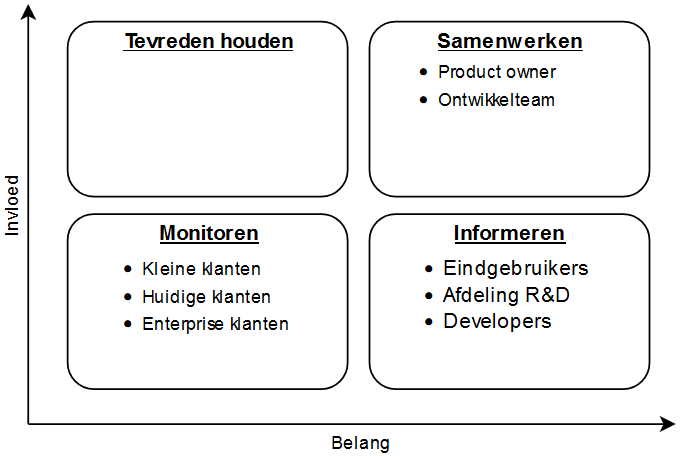
\includegraphics[scale=0.4]{StakeholdersInvloedMatrix}
\subsection{Relatie tussen stakeholders}
\todo[inline]{inleidend stukje text product owner vervangen in opdracht gever?}
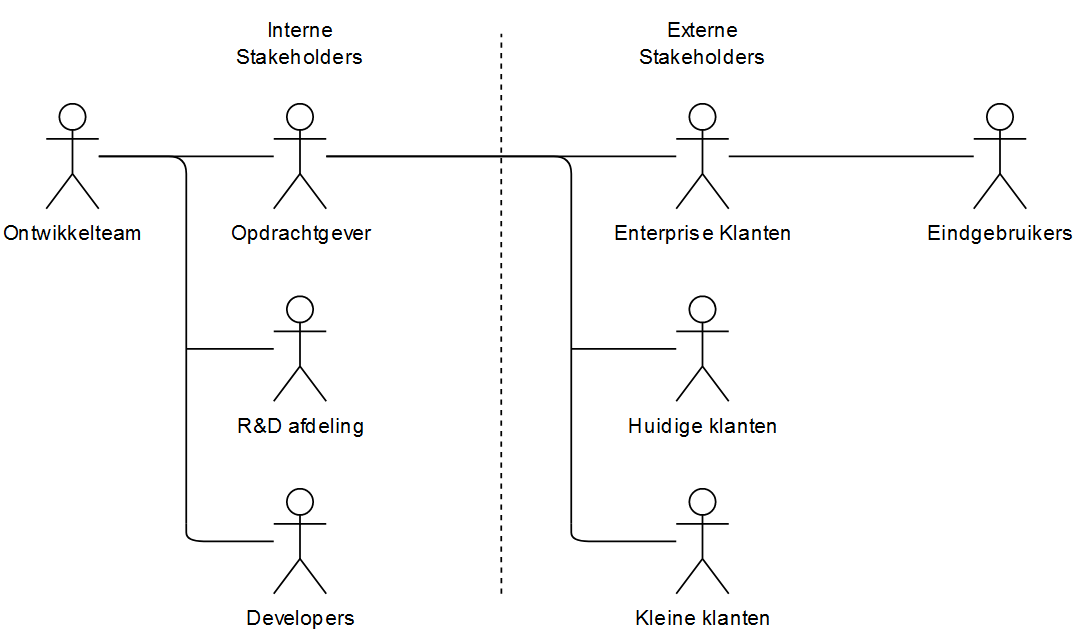
\includegraphics[scale=0.4]{StakeholdersRelatieDiagram}

